\section{Experiments}
\label{sec:experiments}

\subsection{Benchmarks and Evaluation}

We evaluate on the LIBERO-based long-tail setting introduced by Beyond the Majority~\cite{zhu2026beyond}. The main simulated benchmark is \liberocorelt{}, a 10-task long-tailed split with three head tasks and seven tail tasks. We also report a controlled \liberocorefull{} counterpart experiment using the same training and evaluation pipeline. Finally, we are constructing \liberospatiallt{}, a new simulated long-tail split from LIBERO-Spatial, to test whether the method generalizes beyond the Core task set. This last experiment is not yet included in the main numerical claims.

Unless otherwise specified, our evaluations use 30 rollouts per task for \liberocorelt{} and 50 rollouts per task for the \liberocorefull{} controlled comparison. We report success rate averaged across tasks. Our current results are single-seed runs; multi-seed evaluation is required before the strongest statistical claims.

\subsection{Main Results}

\begin{table}[t]
  \centering
  \caption{Main \liberocorelt{} comparison. Reported baselines, re-sampling results, APA ablations, and APA full results are from Beyond the Majority~\cite{zhu2026beyond}. RBTAD is our current single-seed evaluation and should be read as controlled evidence rather than a final multi-seed protocol result.}
  \label{tab:main}
  \begin{tabular}{llc}
    \toprule
    Family & Method & Success rate \\
    \midrule
    BC & Original distribution & 26.5\% \\
    Re-sampling & $q=0.75$ & 25.1\% \\
    Re-sampling & $q=0.50$ & 25.1\% \\
    Re-sampling & $q=0.25$ & 27.1\% \\
    APA ablation & Formatting only & 26.0\% \\
    APA ablation & Augmentation only & 26.9\% \\
    APA & Formatting + augmentation & 36.1\% \\
    Ours & RBTAD & \textbf{40.0\%} \\
    \bottomrule
  \end{tabular}
\end{table}

On \liberocorelt{}, RBTAD reaches 40.0\%. Table~\ref{tab:main} places this result against the full set of reported baselines rather than only APA: conventional re-sampling peaks at 27.1\%, individual APA components remain near the BC baseline, and full APA reaches 36.1\%. We do not present the 40.0\% result as a final SOTA claim yet because our run is currently single-seed and our local pipeline has not fully reproduced the reported three-seed protocol. The result is nevertheless meaningful: it is obtained without generated approach demonstrations, without object grafting, and without inference-time architectural changes.

\begin{table}[t]
  \centering
  \caption{Controlled counterpart results outside the main \liberocorelt{} benchmark. These runs use our local pipeline with the same seed and 50 rollouts per task.}
  \label{tab:controlled_full}
  \begin{tabular}{llc}
    \toprule
    Dataset & Method & Success rate \\
    \midrule
    \multirow{2}{*}{\liberocorefull{}}
      & BC baseline & 43.0\% \\
      & TCAD-trained & \textbf{50.0\%} \\
    \midrule
    \liberospatiallt{} & RBTAD & In progress \\
    \bottomrule
  \end{tabular}
\end{table}

\begin{figure}[t]
  \centering
  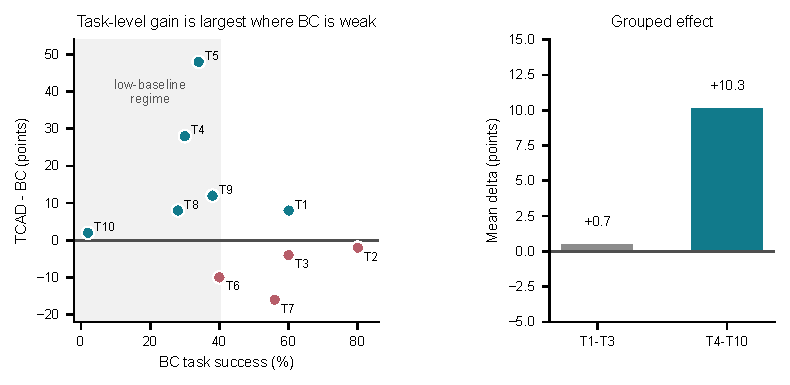
\includegraphics[width=0.78\linewidth]{figures/rbtad/fig3_corefull_delta_analysis.pdf}
  \caption{Task-level analysis on \liberocorefull{}. Rather than duplicating the per-task table, this plot relates each task's baseline success rate to the TCAD gain. Improvements concentrate in the low-baseline regime and in tasks 4--10, while several already strong tasks are flat or slightly worse.}
  \label{fig:corefull_control}
\end{figure}

The \liberocorefull{} controlled comparison in Table~\ref{tab:controlled_full} and Figure~\ref{fig:corefull_control} gives a cleaner within-pipeline signal. Using the same seed and evaluation budget, the baseline reaches 43.0\%, while the TCAD-trained policy reaches 50.0\%. This suggests that the action-discrimination objective is not only exploiting the exact long-tail split; it can also help difficult task-conditioned action boundaries in the full counterpart dataset.

\subsection{Per-Task Results}

\begin{table}[t]
  \centering
  \caption{Local per-task \liberocorelt{} comparison with 30 rollouts per task. The local BC baseline is a reproduced evaluation checkpoint rather than the three-seed number reported in Beyond the Majority.}
  \label{tab:corelt_tasks}
  \begin{tabular}{lcccccccccc}
    \toprule
    Method & T1 & T2 & T3 & T4 & T5 & T6 & T7 & T8 & T9 & T10 \\
    \midrule
    Local BC & .63 & .37 & .23 & .40 & .43 & .23 & .00 & .07 & .03 & .00 \\
    RBTAD & .60 & .53 & .43 & .57 & .50 & .30 & .60 & .13 & .37 & .00 \\
    \bottomrule
  \end{tabular}
\end{table}

The per-task results show a mixed but informative pattern. On \liberocorelt{}, RBTAD improves several tail tasks that the local BC baseline nearly fails, especially T7 and T9, but it still does not solve T10. In \liberocorefull{}, Figure~\ref{fig:corefull_control} shows that the overall gain is not driven by uniform improvement across all tasks. Several difficult object-relation tasks improve substantially, while some already strong tasks slightly decrease. This is consistent with the intended role of TCAD: it sharpens task-conditioned action boundaries rather than simply increasing all success rates uniformly.

\subsection{Implementation Details}

We fine-tune miniVLA-style checkpoints using the same model architecture and inference pathway as the baseline. RBTAD uses two GPUs during training and evaluation in our screening runs, avoiding four-GPU saturation. The \liberocorelt{} RBTAD configuration uses $\lambda=0.1$, $\rho=0.5$, margin $m=0.2$, rare threshold $\tau=9$, and rare BC weight $w_{\mathrm{rare}}=3.0$. The \liberocorefull{} TCAD run disables rare weighting and applies the TCAD signal more broadly, because the split is not long-tailed.



